
% Nineteen chapter ----------------------------------------------------
\chapter*{Nineteen}
\addcontentsline{toc}{chapter}{Nineteen}

\begin{flushright}
\parbox{0.8\textwidth}{
\emph{The truth is at the beginning of anything and its end are alike touching. \\
\hspace*{\fill}{\textperiodcentered \textperiodcentered \textperiodcentered \hspace*{0.2em} Yoshida Kenko} } }
\end{flushright}

\noindent
Nineteen is chess variant which is played on 18 x 18 board, with
light gold-yellow and white fields and gold-yellow and dark gray
pieces. Star colors are the same as for ordinary pieces, i.e.
gold-yellow and dark gray. In algebraic notation, columns are
enumerated from 'a' to 'r', and rows are enumerated from '1' to '18'.
A new piece is introduced, Star.

\textbf{\huge{TODO :: Star colors !!!}} % TODO :: FIX ME !!!

\clearpage % ..........................................................

\section*{Star}
\addcontentsline{toc}{section}{Star}

\noindent
\begin{wrapfigure}{l}{0.4\textwidth}
\centering
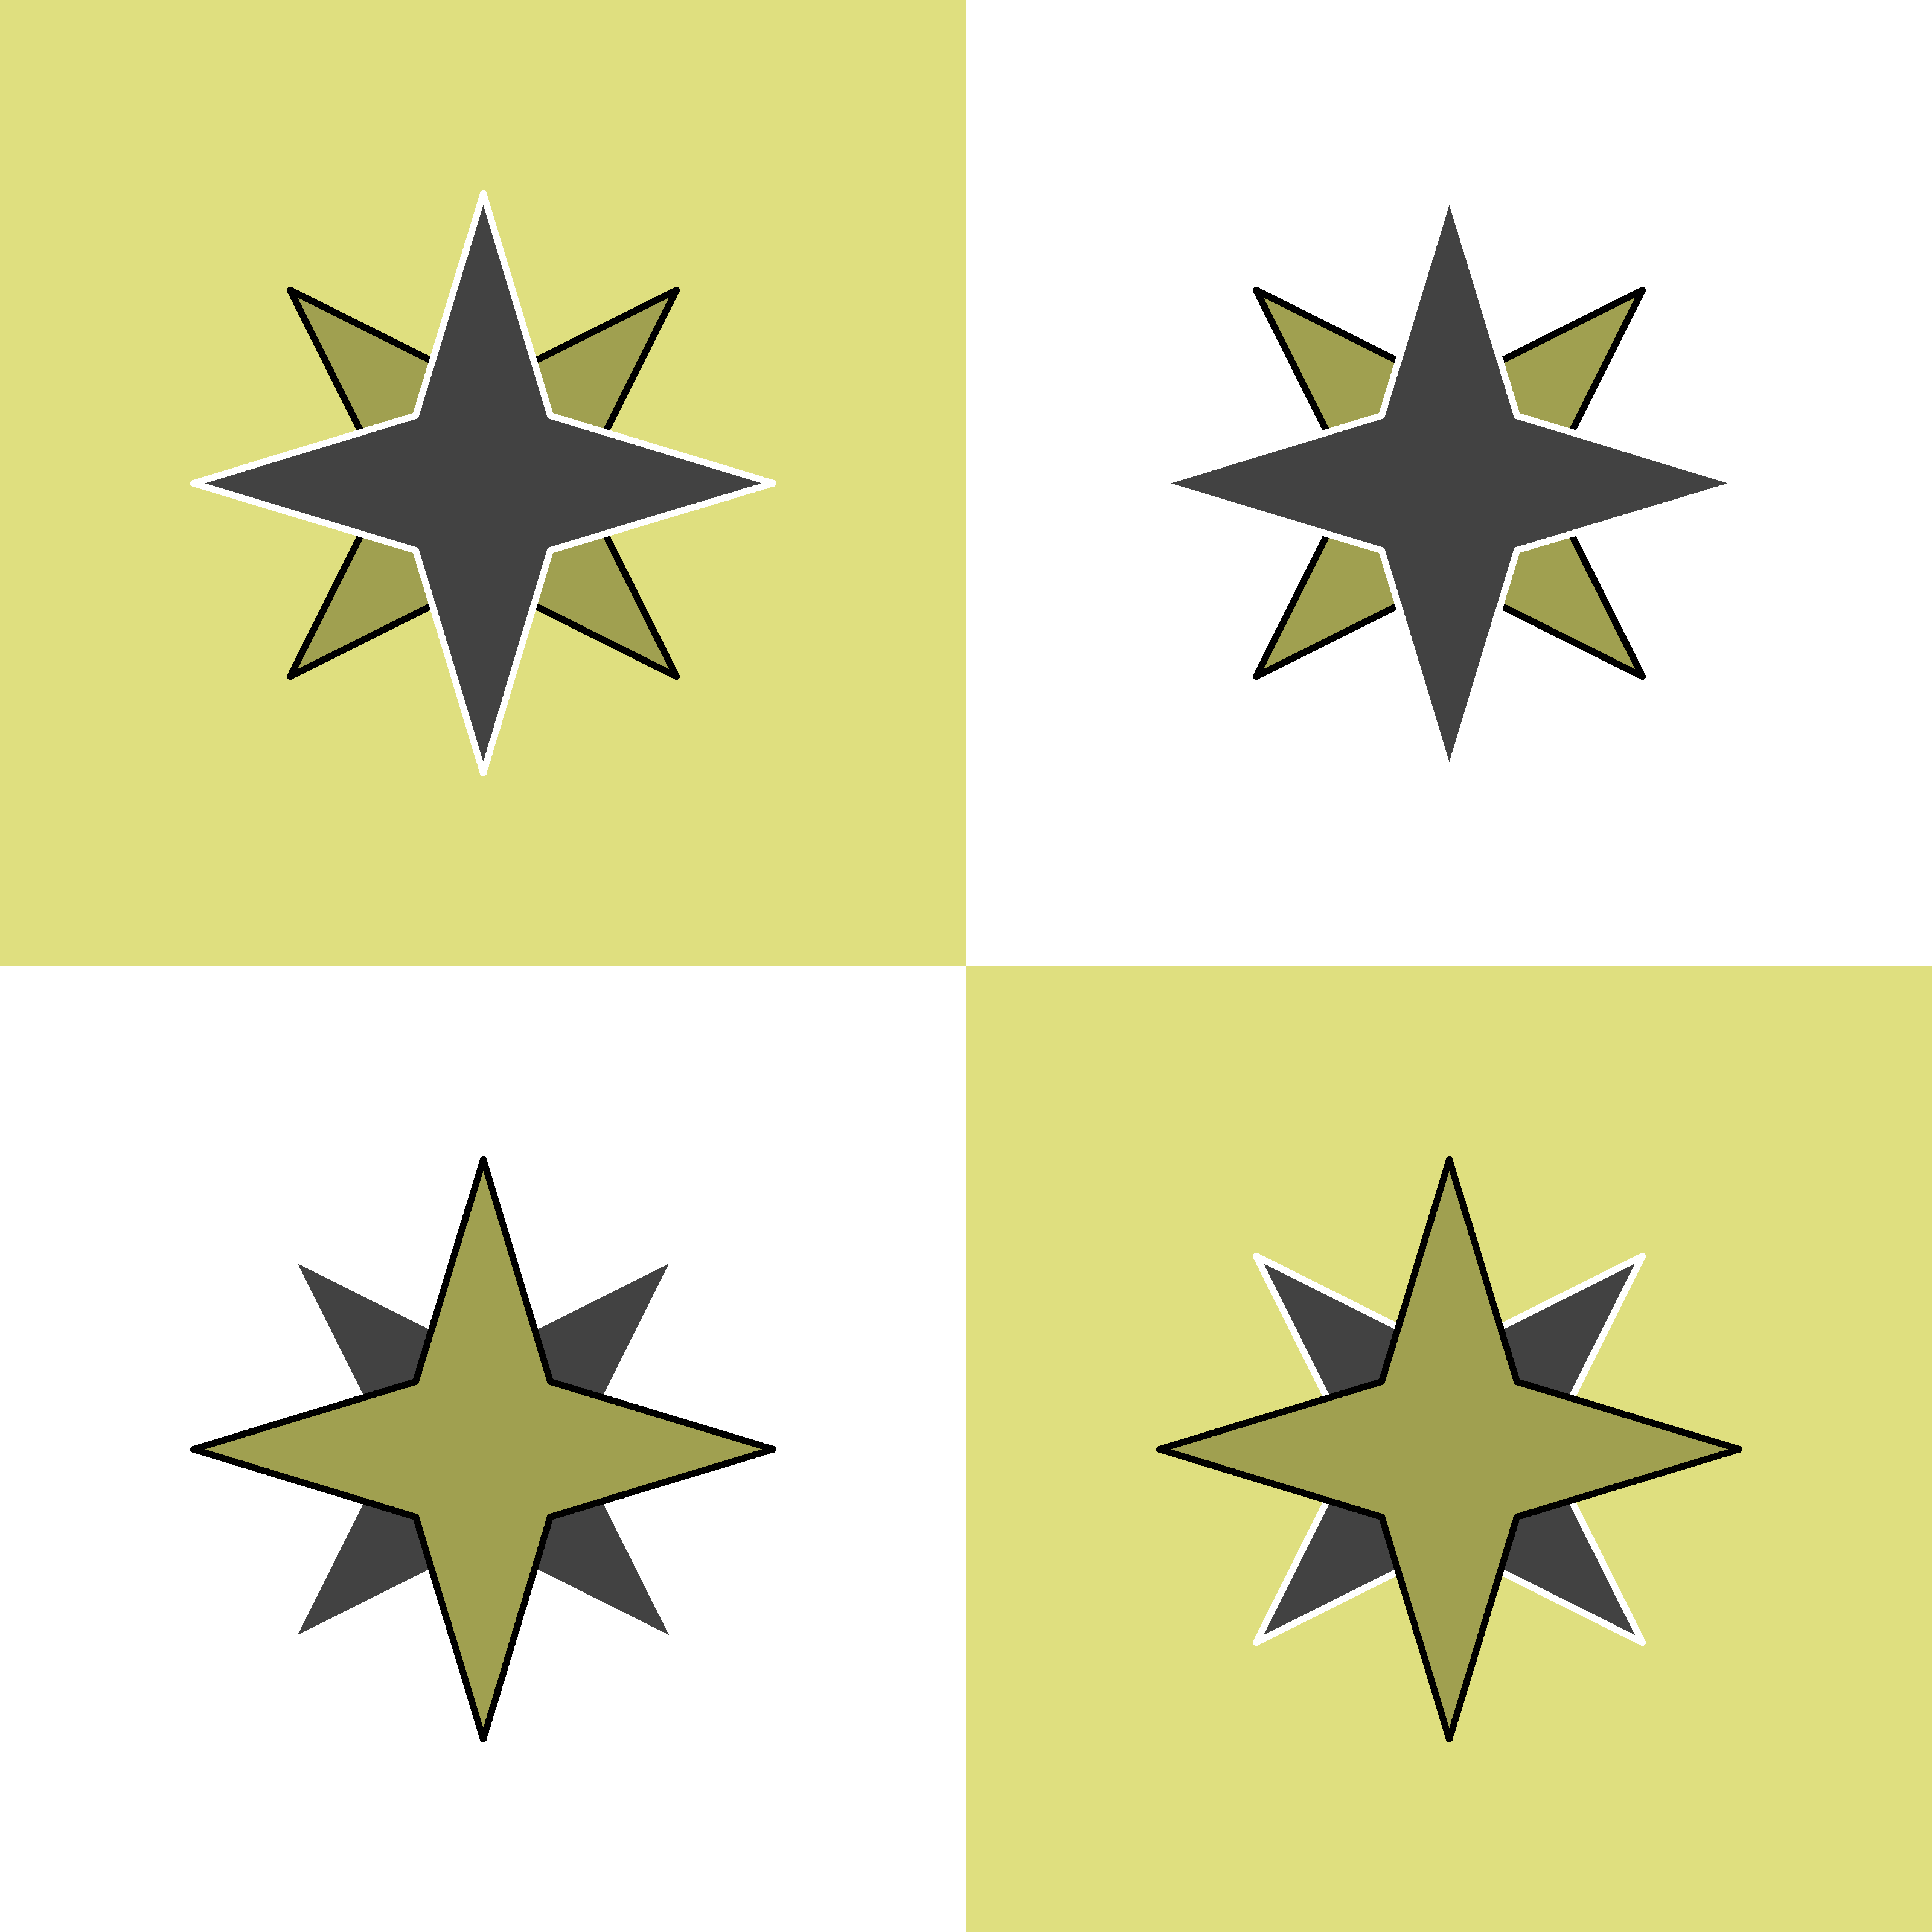
\includegraphics[width=0.4\textwidth, keepaspectratio=true]{pieces/11_star.png}
\caption{Star}
\label{fig:11_star}
\end{wrapfigure}

Pawn cannot be promoted to Star.

Star cannot be activate by Pyramid nor Wave.

\clearpage % ..........................................................

\section*{Initial setup}
\addcontentsline{toc}{section}{Initial setup}

Initial setup can be seen in image below:

\noindent
% \begin{figure}[t]
\begin{figure}[h]
\includegraphics[width=1.0\textwidth, keepaspectratio=true]{boards/12_nineteen.png}
\caption{Nineteen board}
\label{fig:12_nineteen}
% \centering
\end{figure}

\clearpage % ..........................................................
% ---------------------------------------------------- Nineteen chapter
